\documentclass[12pt,mathserif,aspectratio=169]{beamer}
\usepackage[brazil]{babel}
\usepackage[utf8]{inputenc}
\usepackage[T1]{fontenc}
\usepackage{lmodern}
\usepackage{latexsym}
\usepackage{amssymb}
\usepackage{amsmath}
\usepackage{mathtools}
\usepackage{graphicx}
\usepackage{url}
\usepackage[portuguese,onelanguage,ruled]{algorithm2e}
\usepackage{hyperref}
\usepackage{ulem}

%%% CODE %%%
\usepackage{listings}
\usepackage{color}

\definecolor{codegreen}{rgb}{0,0.6,0}
\definecolor{codegray}{rgb}{0.5,0.5,0.5}
\definecolor{codepurple}{rgb}{0.58,0,0.82}
\definecolor{backcolour}{rgb}{0.95,0.95,0.92}

\lstdefinestyle{mystyle}{
	backgroundcolor=\color{backcolour},
	commentstyle=\color{codegreen},
	keywordstyle=\color{magenta},
	numberstyle=\tiny\color{codegray},
	stringstyle=\color{codepurple},
	basicstyle=\footnotesize,
	breakatwhitespace=false,
	breaklines=true,
	captionpos=b,
	keepspaces=true,
	numbers=left,
	numbersep=5pt,
	showspaces=false,
	showstringspaces=false,
	showtabs=false,
	tabsize=2
}

\lstset{style=mystyle}
%%% CODE %%%

\usecolortheme{whale}
\useoutertheme{infolines}
\setbeamertemplate{headline}[default]
\setbeamertemplate{caption}{\insertcaption}
\setbeamertemplate{navigation symbols}{}
\centering

\title[Introdução ao Aprendizado de Máquina]{Introdução ao Aprendizado de Máquina}
\author[Prof. Erneson A. Oliveira]{Prof. Erneson A. Oliveira$^*$}
\institute[MBACD-UNIFOR]{MBA em Ciência de Dados\\Universidade de Fortaleza}
\date{27 de Março de 2021}

\begin{document}

%%% TITLE %%%
\begin{frame}
    \vspace{1.0cm}
    \titlepage
    \vspace{-1.5cm}
    
    \begin{figure}
        \begin{minipage}{0.4\paperwidth}
            \vspace{1.75cm}
            \begin{flushleft}
                {\tiny $^*$ erneson@unifor.br}
            \end{flushleft}
        \end{minipage}
        \hfill
        \begin{minipage}{0.4\paperwidth}
            \vspace{-0.5cm}
            \begin{flushright}
                \includegraphics[width=0.2\paperwidth]{fig/UNIFOR.jpg}
            \end{flushright}
        \end{minipage}
    \end{figure}
\end{frame}
%%% TITLE %%%

%%% SLIDE %%%
\begin{frame}
	\Large Aula 3 - Desafios de Aprendizado de Máquina
	\begin{figure}
		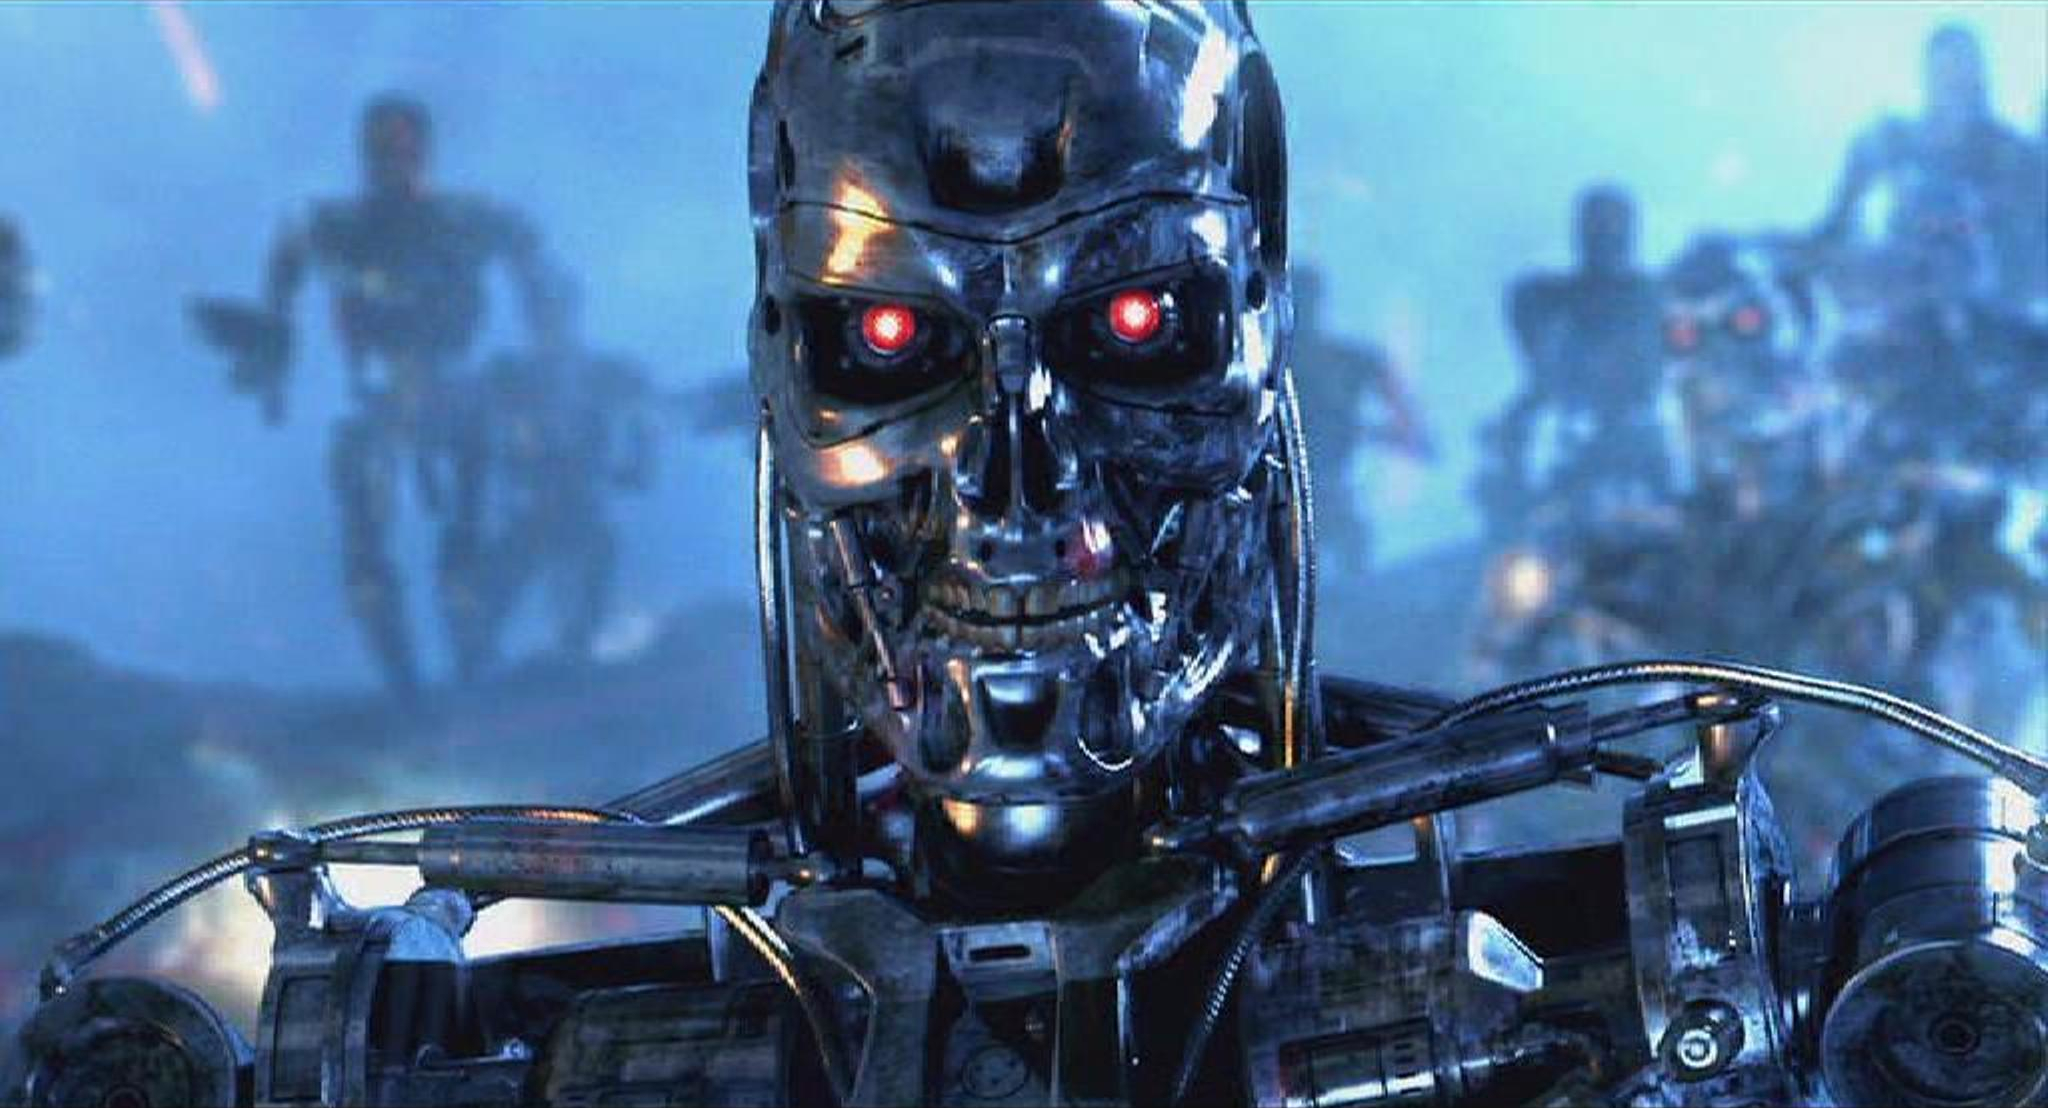
\includegraphics[width=0.8\paperwidth]{fig/skynet.jpg}
	\end{figure}
\end{frame}
%%% SLIDE %%%

%%% SLIDE %%%
\begin{frame}{Exemplo}
    \begin{figure}
	    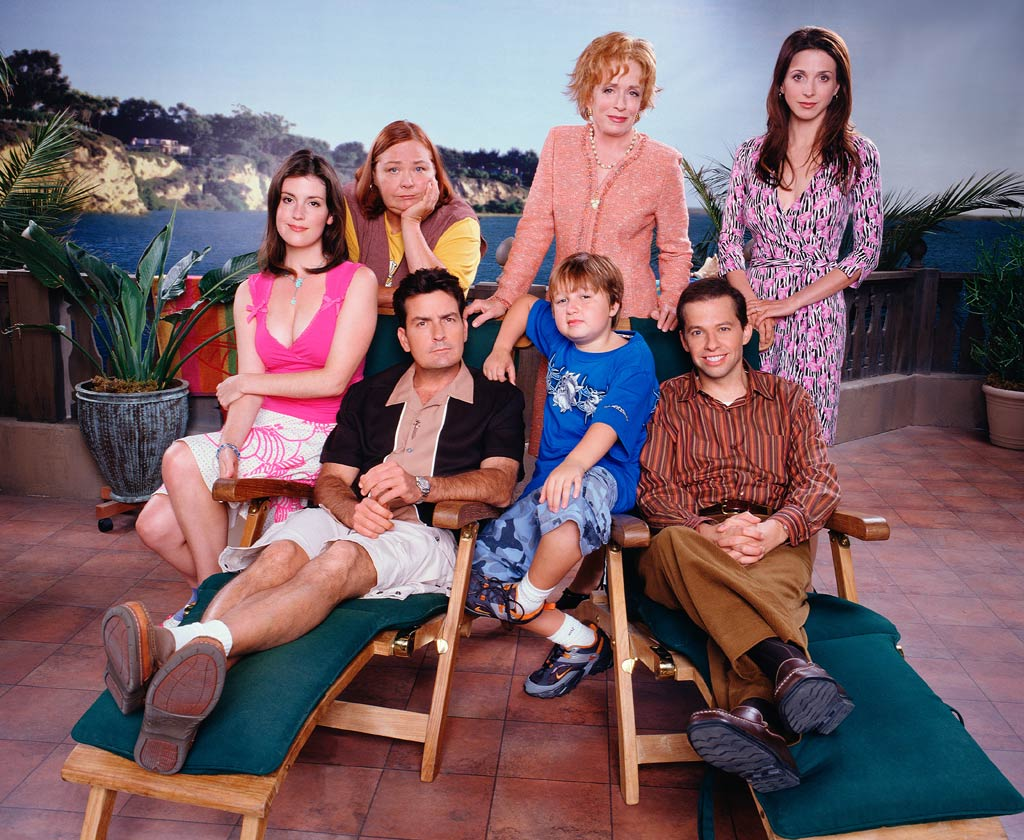
\includegraphics[width=0.45\paperwidth]{fig/taahm.jpg}
	    \caption{Como prever preços de habitações?}
    \end{figure}
\end{frame}
%%% SLIDE %%%

%%% SLIDE %%%
\begin{frame}
    \Huge Quais são os principais desafios em AM?
\end{frame}
%%% SLIDE %%%

%%% SLIDE %%%
\begin{frame}
    \Huge Quantidade insuficiente de dados no conjunto de treinamento
\end{frame}
%%% SLIDE %%%

%%% SLIDE %%%
\begin{frame}{Quantidade insuficiente de dados no conjunto de treinamento}
    \only<1>{
        \begin{minipage}{0.45\paperwidth}
    	    \begin{figure}
                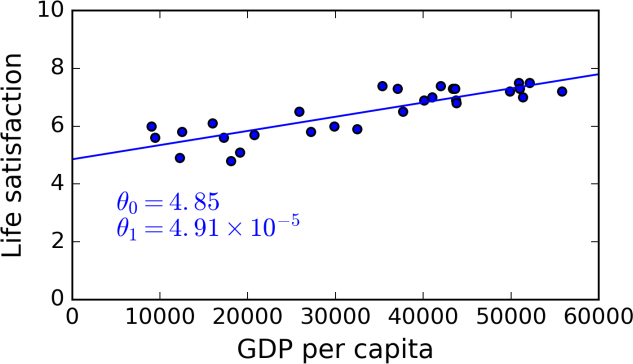
\includegraphics[width=0.9\textwidth]{fig/fig1_19.jpg}
    	    \end{figure}
        \end{minipage}
        \begin{minipage}{0.45\paperwidth}
            \begin{figure}
                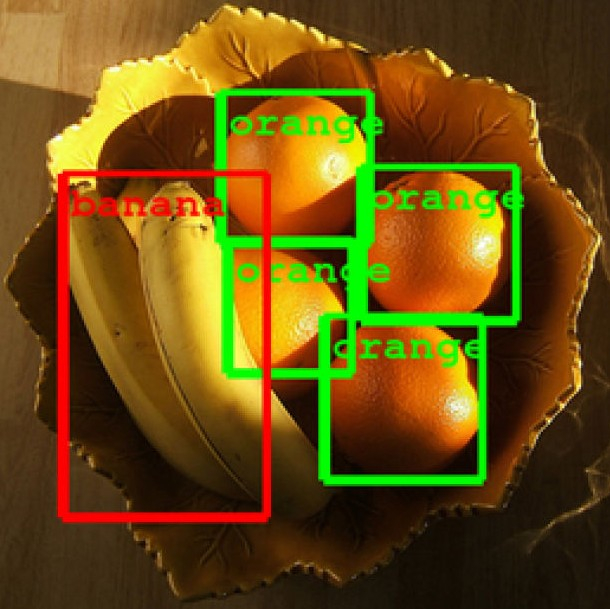
\includegraphics[width=0.9\textwidth]{fig/object_recognition.jpg}
    	    \end{figure}
        \end{minipage}
        
        Problemas simples $\times$ Problemas complicados
	}
	
	\only<2>{
        \begin{minipage}{0.45\paperwidth}
    	    \begin{figure}
                
\includegraphics[width=0.9\textwidth]{fig/paper_banko.jpg}
    	    \end{figure}
        \end{minipage}
        \begin{minipage}{0.45\paperwidth}
            \begin{figure}
                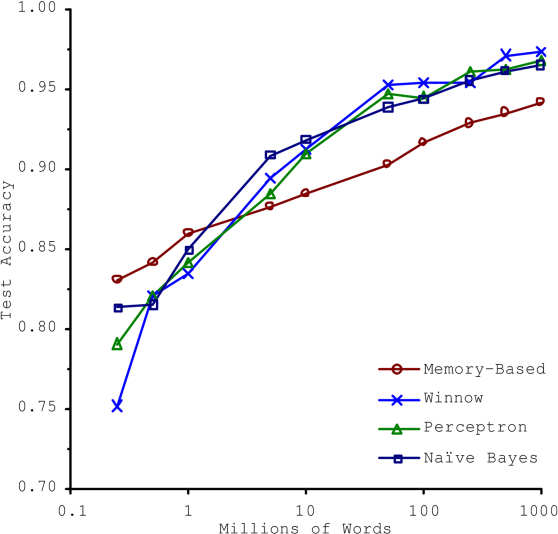
\includegraphics[width=0.9\textwidth]{fig/fig1_20.jpg}
    	    \end{figure}
        \end{minipage}
        
        Dados $\times$ Algoritmos
	}
	
	\only<3>{
	    \begin{figure}
            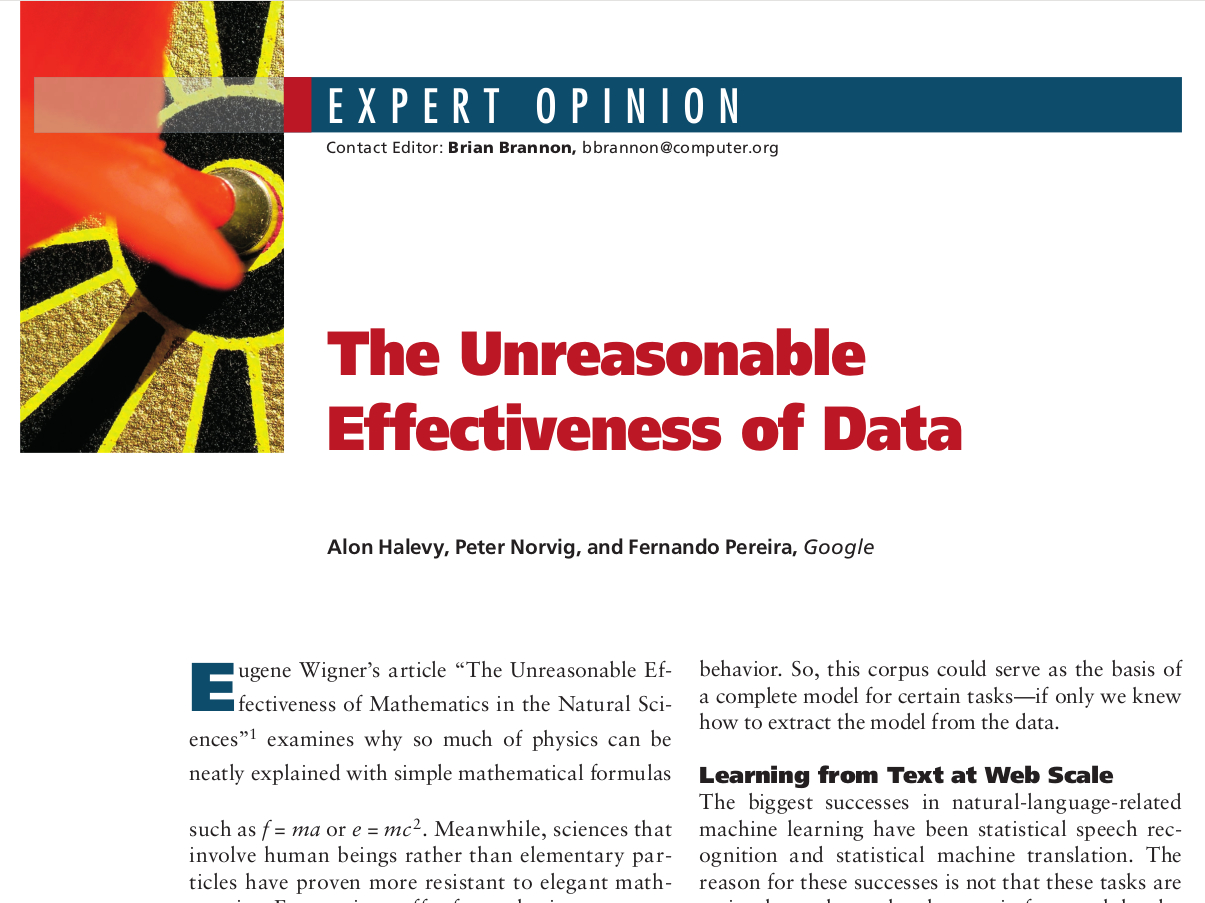
\includegraphics[width=0.5\textwidth]{fig/paper_halevy.jpg}
	    \end{figure}
        
        Dados são mais importantes do que algoritmos?
	}
\end{frame}
%%% SLIDE %%%

%%% SLIDE %%%
\begin{frame}
	\Huge Dados de treinamento não-representativos
\end{frame}
%%% SLIDE %%%

%%% SLIDE %%%
\begin{frame}{Dados de treinamento não-representativos}
    \only<1>{
        \begin{figure}
            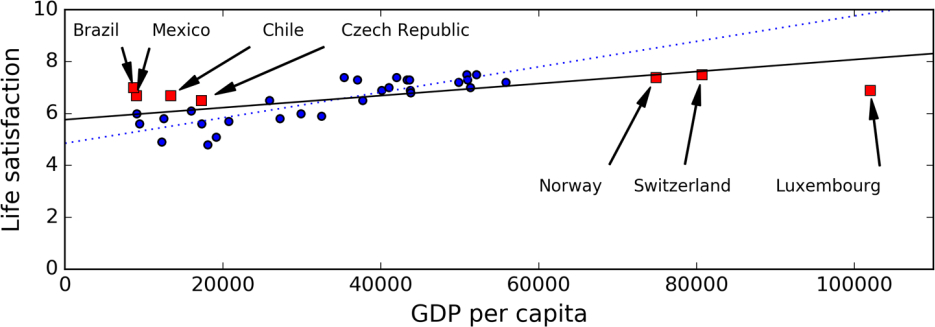
\includegraphics[width=0.8\textwidth]{fig/fig1_21.jpg}
	    \end{figure}
        
        Dados de treinamento devem ser representativos para novos casos (ruído na amostragem)!
	}
	
	\only<2>{
        \begin{minipage}{0.40\paperwidth}
    	    \begin{figure}
                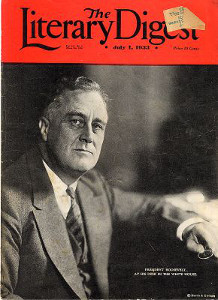
\includegraphics[width=0.65\textwidth]{fig/literary_digest.jpg}
    	    \end{figure}
        \end{minipage}
        \begin{minipage}{0.50\paperwidth}
            \begin{figure}
                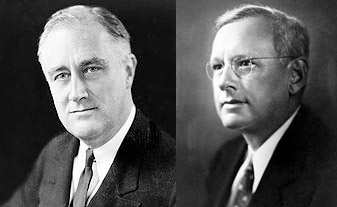
\includegraphics[width=0.9\textwidth]{fig/landon_roosevelt.jpg}
                \caption{Eleições dos EUA (1936): Roosevelt $\times$ Landon}
    	    \end{figure}
        \end{minipage}
        
        \begin{itemize}
            \item Viés na amostragem e viés de não-resposta.
        \end{itemize}
	}
\end{frame}
%%% SLIDE %%%

%%% SLIDE %%%
\begin{frame}
	\Huge Qualidade baixa dos dados
\end{frame}
%%% SLIDE %%%

%%% SLIDE %%%
\begin{frame}{Qualidade baixa dos dados}
    \begin{table}%[tbhp]
        \centering
        \begin{tabular}{c|c|c|c|c|c}
        {\bf Modelo}  & {\bf Quilometragem (km)} & {\bf Ano}    & {\bf Marca}      & \dots  & {\bf Valor (R\$)}\\
        \hline
        COROLLA       & $1.000$                  & 2019         & Toyota           & \dots  & $60\;000\;000$\\
        Fusquinha     & $100\;000$               & 1984         & V0lkswagem       & \dots  & $2\;000$\\
        Onix 2017     & $15,000$                 & 2017         & Chevrolet        & \dots  & $30\;000$\\
        \vdots        & \vdots                   & \vdots       & \vdots           & \vdots & \vdots\\
        Duster        & $10\;000$                & 2218         & Renault          & \dots  & $45.000$
        \end{tabular}
    \end{table}
    
    \begin{itemize}
        \item Mineração, higienização e padronização dos dados.
    \end{itemize}
\end{frame}
%%% SLIDE %%%

%%% SLIDE %%%
\begin{frame}
	\Huge Características irrelevantes
\end{frame}
%%% SLIDE %%%

%%% SLIDE %%%
\begin{frame}{Características irrelevantes}
    \begin{table}%[tbhp]
        \centering
        \begin{tabular}{c|c|c|c|c|c}
        {\bf Modelo}  & {\bf Quilometragem (km)} & \sout{{\bf Ano}}    & {\bf Marca}      & \dots  & {\bf Valor (R\$)}\\
        \hline
        Corolla       & $1\;000$                 & \sout{2019}         & Toyota           & \dots  & $60\;000$\\
        Fusca         & $100\;000$               & \sout{1984}         & Volkswagem       & \dots  & $2\;000$\\
        Onix          & $15\;000$                & \sout{2017}         & Chevrolet        & \dots  & $30\;000$\\
        \vdots        & \vdots                   & \vdots              & \vdots           & \vdots & \vdots\\
        Duster        & $10\;000$                & \sout{2018}         & Renault          & \dots  & $45\;000$
        \end{tabular}
    \end{table}
    
    \begin{itemize}
        \item Engenharia de características: Seleção, extração, criação de características.
    \end{itemize}
\end{frame}
%%% SLIDE %%%

%%% SLIDE %%%
\begin{frame}
	\Huge Em suma, para dados...
\end{frame}
%%% SLIDE %%%

%%% SLIDE %%%
\begin{frame}{Em suma, para dados...}
    \begin{figure}
        
\includegraphics[width=0.7\textwidth]{fig/gigo0.pdf}
        \caption{{\it Garbage in, garbage out}!}
    \end{figure}
\end{frame}
%%% SLIDE %%%

%%% SLIDE %%%
\begin{frame}
	\Huge Sobreajuste do conjunto de treinamento
\end{frame}
%%% SLIDE %%%

%%% SLIDE %%%
\begin{frame}{Sobreajuste do conjunto de treinamento}
    \only<1>{
        \begin{minipage}{0.45\paperwidth}
    	    \begin{itemize}
    	        \item Sobreajuste (ou {\it Overfitting}): Acontece quando o SAM tem bom desempenho apenas no conjunto de treinamento, {\it i.e.} quando o SAM é muito complexo em relação ao conjunto de treinamento.
            \end{itemize}
        \end{minipage}
        \begin{minipage}{0.45\paperwidth}
            \begin{figure}
                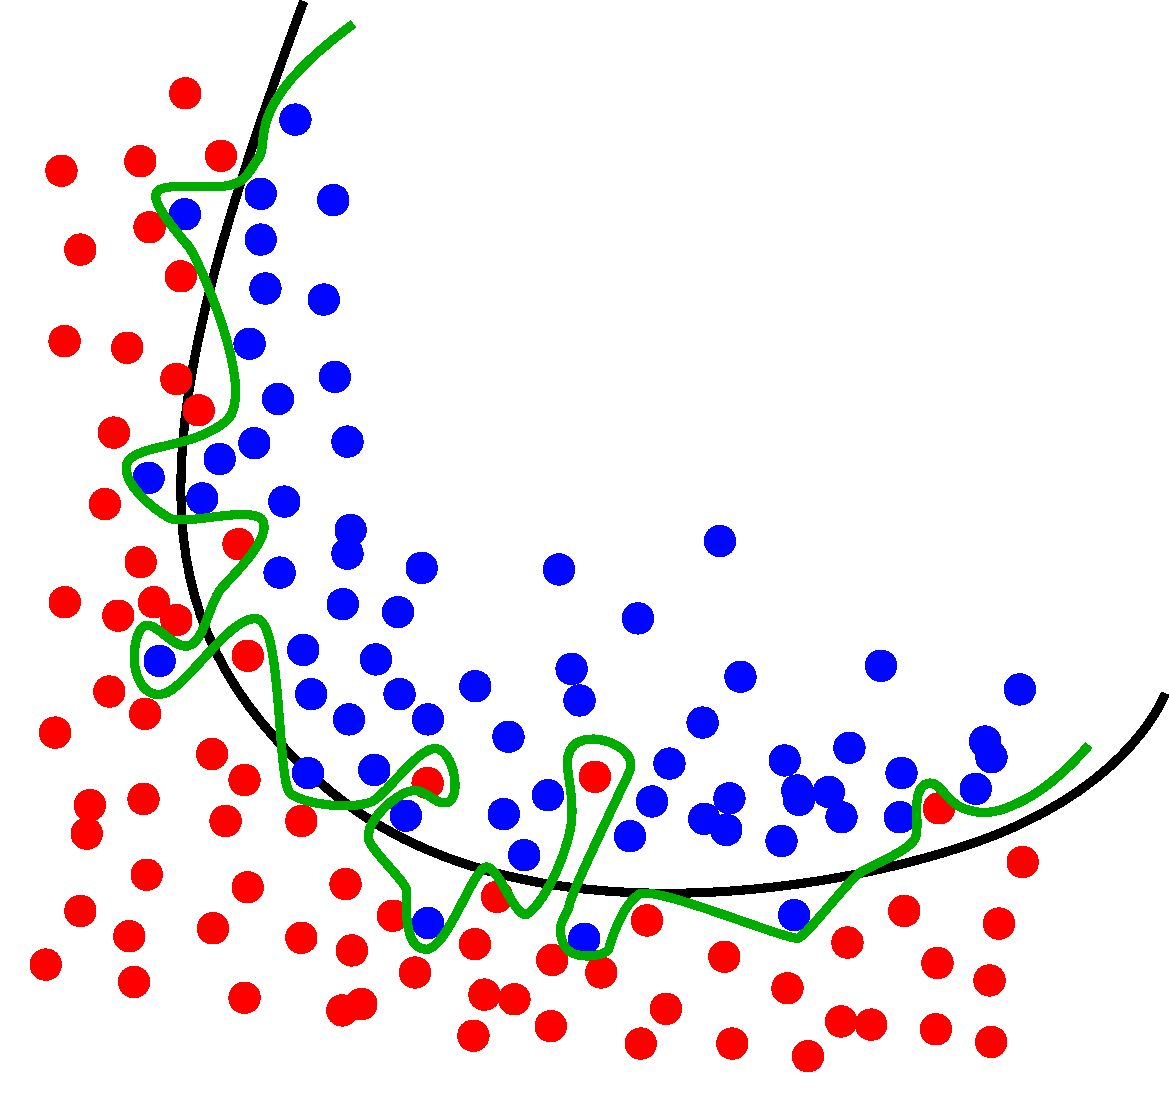
\includegraphics[width=1.0\textwidth]{fig/overfitting.pdf}
            \end{figure}
        \end{minipage}
    }
    
    \only<2>{
        \begin{figure}
            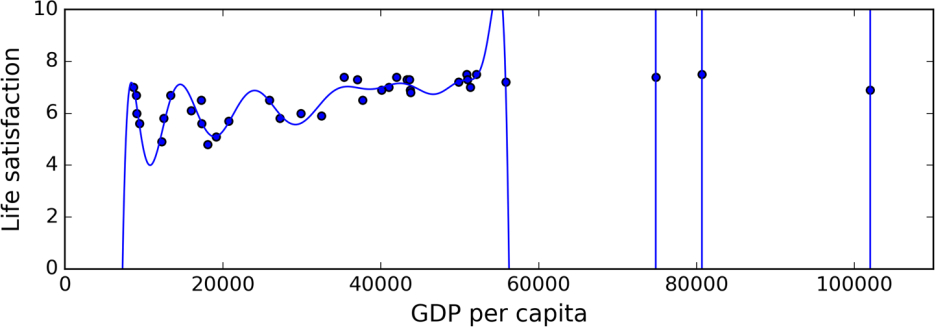
\includegraphics[width=0.8\textwidth]{fig/fig1_22.jpg}
            \caption{Sobreajuste do conjunto de treinamento!}
        \end{figure}
    }
    
    \only<3>{
        \begin{itemize}
            \item Regularização: Imposição de restrições, controladas pelos hiperparâmetros, ao AA para tornar o SAM mais simples.
        \end{itemize}
        
        \begin{figure}
            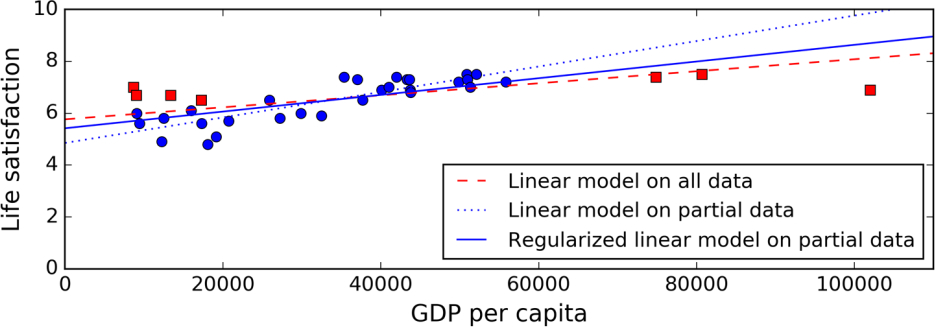
\includegraphics[width=0.8\textwidth]{fig/fig1_23.jpg}
            \caption{Regularização reduz os riscos de sobreajustes!}
        \end{figure}
    }
    
    \only<4>{
        \large Como resolver o sobreajuste?
    }
    
    \only<5-9>{
		\begin{enumerate}
			\uncover<5->{\item Utilizar um modelo mais simples;}
			\uncover<6->{\item Reduzir o número de atributos;}
			\uncover<7->{\item Restrigir o modelo;}
			\uncover<8->{\item Adquirir mais dados;}
			\uncover<9->{\item Reduzir o ruído do conjunto de treinamento.}
		\end{enumerate}
	}
\end{frame}
%%% SLIDE %%%

%%% SLIDE %%%
\begin{frame}
	\Huge Subajuste do conjunto de treinamento
\end{frame}
%%% SLIDE %%%

%%% SLIDE %%%
\begin{frame}{Subajuste do conjunto de treinamento}
    \only<1>{
        \begin{minipage}{0.45\paperwidth}
	        \begin{itemize}
	            \item Subajuste ({\it Underfitting}): Acontece quando o SAM não tem bom desempenho nem mesmo no conjunto de treinamento, {\it i.e.} quando o SAM é muito simples em relação ao conjunto de treinamento.
            \end{itemize}
        \end{minipage}
        \begin{minipage}{0.45\paperwidth}
            \begin{figure}
                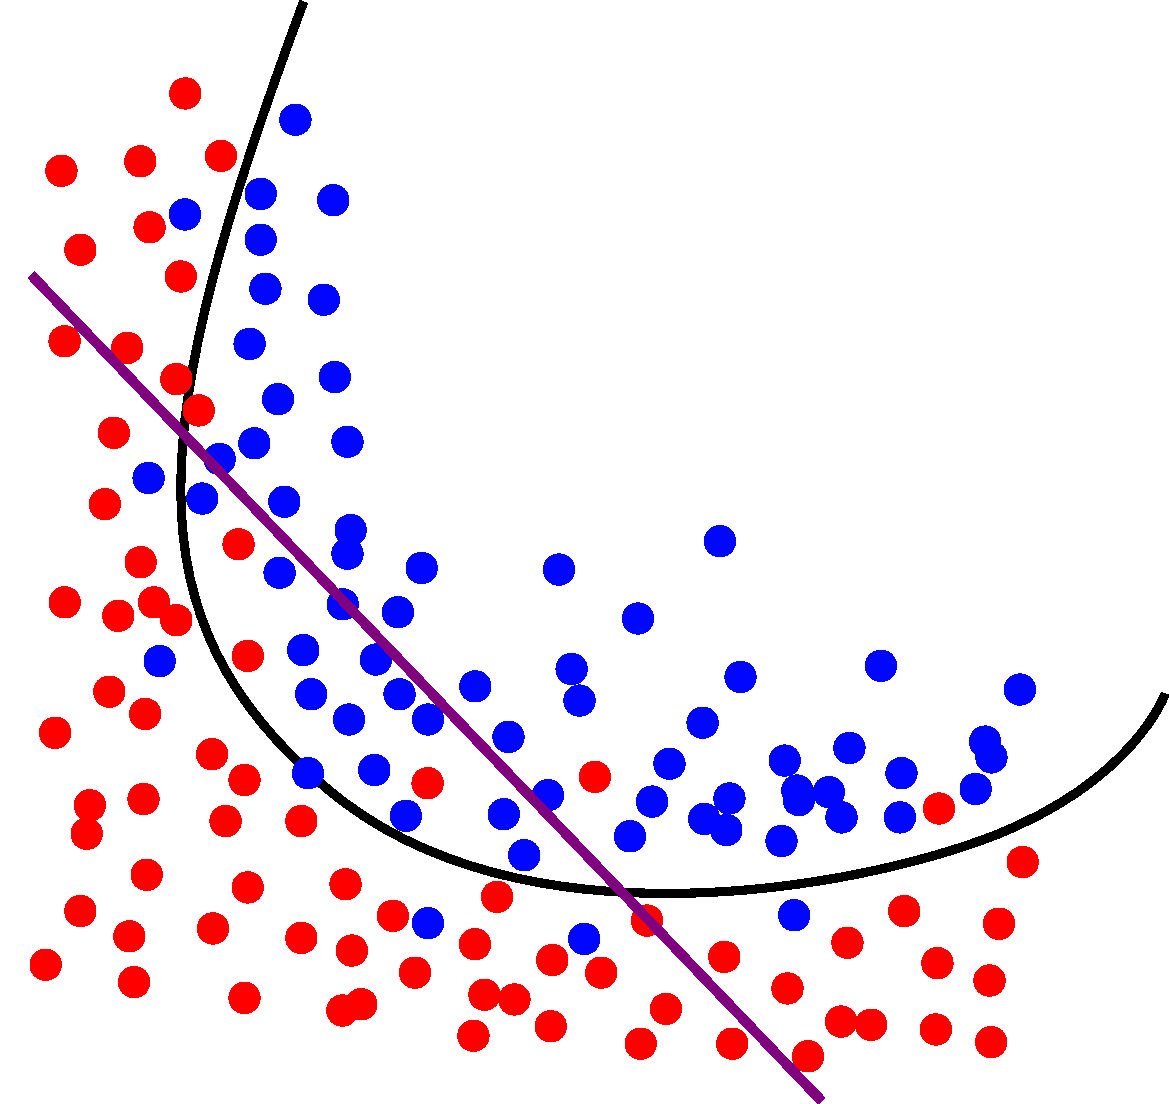
\includegraphics[width=1.0\textwidth]{fig/underfitting.pdf}
            \end{figure}
        \end{minipage}
    }
    
    \only<2>{
        \large Como resolver o subajuste?
    }
    
    \only<3-5>{
		\begin{enumerate}
			\uncover<3->{\item Utilizar um modelo mais poderoso;}
			\uncover<4->{\item Escolher atributos melhores;}
			\uncover<5->{\item Reduzir o número de restrições.}
		\end{enumerate}
	}
\end{frame}
%%% SLIDE %%%

%%% SLIDE %%%
\begin{frame}
	\Huge Conjunto de teste e conjunto de validação
\end{frame}
%%% SLIDE %%%

%%% SLIDE %%%
\begin{frame}{Conjunto de teste e conjunto de validação}
    \only<1>{
        \begin{itemize}
            \item Conjunto de treinamento: Dados usados para ajustar os parâmetros do SAM;
            \item Erro de treinamento.
        \end{itemize}
        
        \begin{figure}
            
\includegraphics[width=1.0\textwidth]{fig/set0.pdf}
        \end{figure}
    }
    
    \only<2-3>{
        \begin{itemize}
            \item Conjunto de teste: Dados usados para fazer a avaliação final do SAM;
            \item Erro de generalização.
        \end{itemize}
        
        \begin{figure}
            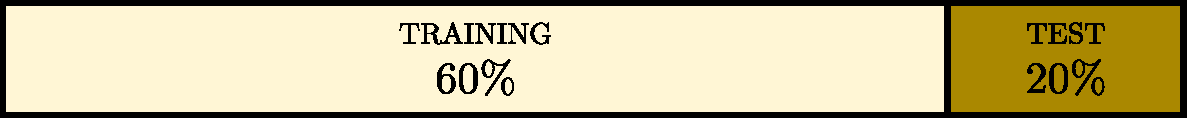
\includegraphics[width=1.0\textwidth]{fig/set1.pdf}
        \end{figure}
        
        \begin{itemize}
            \uncover<3->{\item Se o erro de treinamento é baixo e erro de generalização é alto, então o SAM está sobreajustado.}
        \end{itemize}
    }
    
    \only<4-6>{
        \begin{itemize}
            \item Conjunto de validação: Dados usados para ajustar os hiperparâmetros do AA e fazer avaliações intermediárias do SAM;
            \item Erro de validação.
        \end{itemize}
        
        \begin{figure}
            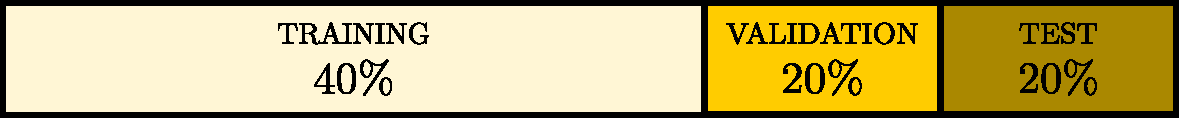
\includegraphics[width=1.0\textwidth]{fig/set2.pdf}
        \end{figure}
        
        \begin{itemize}
            \uncover<5->{\item Se o erro de treinamento é baixo e erro de validação é alto, então o SAM está sobreajustado;}
            \uncover<6->{\item Se os erros de treinamento e validação são baixos e erro de generalização é alto, então o SAM está sobreajustado.}
        \end{itemize}
    }
    
    \only<7>{
        \begin{itemize}
            \item Validação cruzada: Avalia a capacidade de generalização de uma análise estatística a partir de um conjunto de dados ({\it e.g.} {\it $k$-Fold}).
        \end{itemize}
        
        \begin{figure}
            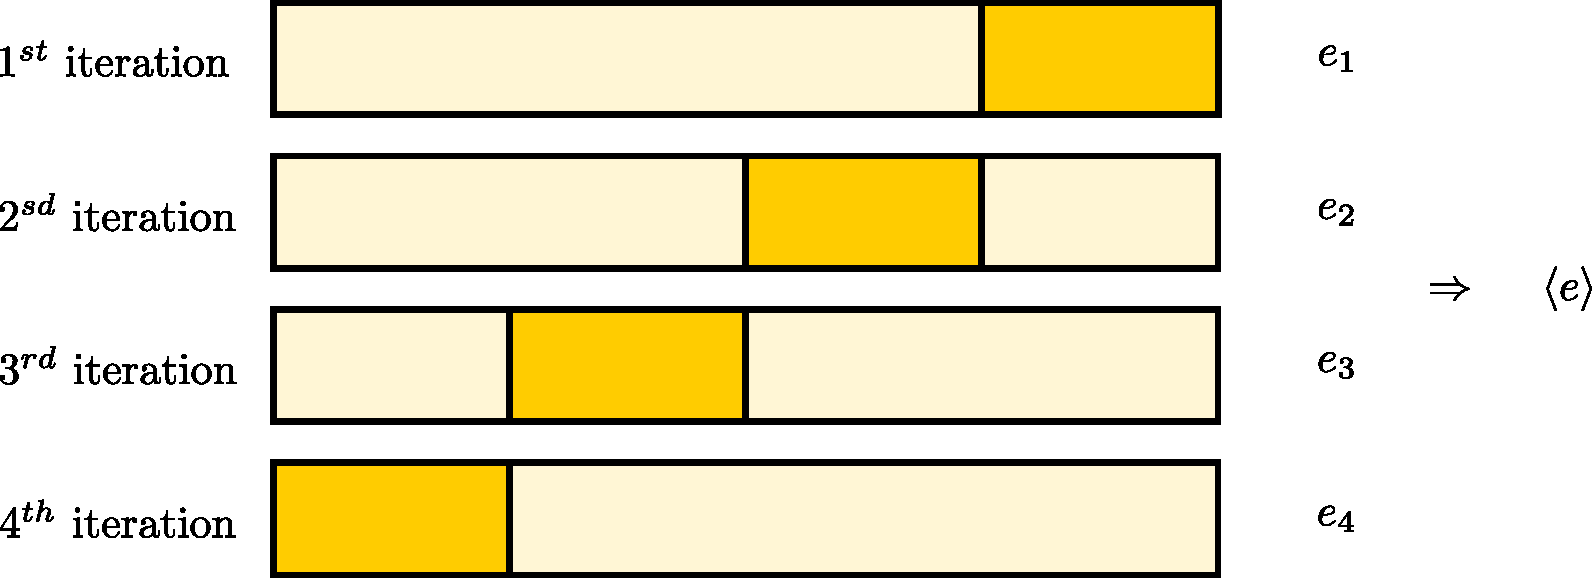
\includegraphics[width=1.0\textwidth]{fig/set3.pdf}
        \end{figure}
    }
\end{frame}
%%% SLIDE %%%

%%% SLIDE %%%
\begin{frame}
	\Huge Em suma, para modelos...
\end{frame}
%%% SLIDE %%%

%%% SLIDE %%%
\begin{frame}{Em suma, para modelos...}
    \begin{figure}
        
\includegraphics[width=0.7\textwidth]{fig/gigo1.pdf}
        \caption{{\it Garbage in, garbage out}!}
    \end{figure}
\end{frame}
%%% SLIDE %%%

%%% SLIDE %%%
\begin{frame}
    \begin{figure}
        
\includegraphics[width=0.9\textwidth]{fig/hastalavistababy.jpg}
    \end{figure}
\end{frame}
%%% SLIDE %%%

\end{document}
